\section{Evaluation}
\label{sec:evaluation}

\subsection{Setup}

\paragraph{Hardware and software.}
Engine: SGLang~\cite{sglang2024}. Model: Qwen2.5-Coder-7B-Instruct.
Temperature 0, decode one token, one warmup and three measured rounds
($235\times 3 = 705$ pairs). Slurm job 137185 on a compute GPU, not a
login or debug node. Prefetch and ordinary prefix reuse are off.
Appendix 30B uses Qwen3-Coder 30B-A3B Instruct (AWQ 4-bit, job 96092)
on the same protocol. Replaying 30B token ids on 7B is invalid.

\paragraph{Dataset.}
SWE-bench Verified~\cite{swebench} trajectories from a 24-task live-agent
run (expanded24). That is a convenience sample of Verified, not the full
500-task split. The 235 target groups are rolling-6 turns, not 235
tasks. Six repositories appear; 20 of 24 instances have at least one
eligible $\Delta\neq 0$ group (Table~\ref{tab:dataset}). The speed
campaign reconstructs exact target prompts and keeps only true-lossy
file-module groups: 421 islands, 361{,}159 copied tokens per measured
round, 48 zero-shift islands dropped at compile time (this is
not a radix TTFT). There are 115 unique source prompts and 235 unique
target prompts. Table~\ref{tab:eval-summary} reports every group in that
compiled PLAN ($235$ groups, $705$ pairs). It is not a further
subsample of the 235, and it is not a 500-task Verified run.

\begin{table}[t]
\centering
\small
\caption{expanded24 dataset card. Groups are rolling-6 turns from 24
Verified tasks, derived from the 7B PLAN (job 137185) plus frozen
trajectories, not a new GPU arm.}
\label{tab:dataset}
\begin{tabular}{lr}
\toprule
\textbf{Item} & \textbf{Count} \\
\midrule
Verified tasks in producer & 24 \\
Repositories & 6 \\
Tasks with eligible groups & 20 \\
Target groups (turns) & 235 \\
True-lossy islands & 421 \\
Dropped $\Delta{=}0$ islands & 48 \\
\bottomrule
\end{tabular}
\end{table}

\paragraph{Baselines.}
Primary: the same SGLang Dense prefill on the same token IDs.
Isolation on the same 235-group PLAN: prefix-only and dual
prefix$+$copy (job 139839, Table~\ref{tab:7b-prefix-on}). Admit clones:
same-engine KVCOMM-style unconstrained copy and CacheBlend-style
$15\%$ boundary recompute (job 137400, Table~\ref{tab:admit-ablation}),
not native stacks. vLLM, LMCache, RelayCaching, Continuum, and Tokencake
are different serving paths; this paper does not crown them.

\paragraph{Metrics.}
Cache-ready target TTFT versus the same engine's Dense: mean, median,
p90, p99, and the ratio of means. Source KV already exists, matching
CacheBlend and KVCOMM. Secondary: paired saving, paired win rate,
copied-token fraction, mechanical copy and fallback counts, one-token
output agreement. One-token agreement is \emph{not} official SWE-bench
resolved. We do not bill a source-inclusive $N$-use speedup.

\subsection{Overall results}

Table~\ref{tab:eval-summary} and Figure~\ref{fig:ttft-cdf}
report the frozen 7B campaign (job 137185, COMPLETE). The same protocol
on a larger AWQ checkpoint is a second serving point, not this table.
Table~\ref{tab:eval-scales} names both jobs; speedups stay in
Table~\ref{tab:eval-summary} and Table~\ref{tab:eval-30b}.

\begin{center}
\small
\captionof{table}{Same file-module protocol at two checkpoints.
Agreement and copy counts only; speedups stay in
Table~\ref{tab:eval-summary} and Table~\ref{tab:eval-30b}.}
\label{tab:eval-scales}
\begin{tabular}{llrr}
\toprule
\textbf{Checkpoint} & \textbf{Job} & \textbf{Agree} & \textbf{Copy} \\
\midrule
Qwen2.5-Coder-7B-Instruct & 137185 & $93.6\%$ & $1684/1684$ \\
Qwen3-Coder 30B-A3B (AWQ) & 96092 & $94.8\%$ & $1684/1684$ \\
\bottomrule
\end{tabular}
\end{center}

\begin{table}[t]
\centering
\small
\caption{Qwen2.5-Coder-7B-Instruct exact-prompt true-lossy file-module
replay (job 137185). Cache-ready TTFT is target generate time after
source KV already exists. One-token agreement is not official resolved.
Not the seven-group dual-island table and not the appendix 30B table.}
\label{tab:eval-summary}
\label{tab:7b-swebench}
% not the seven-group dual-island isolation; see tab:7b-dual-island.
\setlength{\tabcolsep}{4pt}
\begin{tabular}{lrr}
\toprule
\textbf{Metric} & \textbf{Dense} & \textbf{\method{}} \\
\midrule
Target groups & 235 & 235 \\
Measured pairs & 705 & 705 \\
Mean prompt tokens & $4433$ & $4433$ \\
Copied tokens (mean) & --- & $1537$ ($33\%$) \\
Islands & --- & $421$ \\
Copy events / planned & --- & $1684/1684$ \\
Fallback events & --- & $0$ \\
$K$ pre-rotations & --- & $421$ \\
Mean TTFT & $585.9$\,ms & $392.7$\,ms \\
Median TTFT & $555$\,ms & $383$\,ms \\
P90 TTFT & $952$\,ms & $586$\,ms \\
P99 TTFT & $1178$\,ms & $819$\,ms \\
Cache-ready speedup & $1.000\times$ & $1.492\times$ \\
Paired saving (mean / med.) & --- & $30.6\%$ / $27.9\%$ \\
Paired win rate & --- & $99.3\%$ \\
One-token agreement & --- & $93.6\%$ \\
Prefetch / prefix reuse & off & off \\
\bottomrule
\end{tabular}
\end{table}

\begin{figure}[t]
\centering
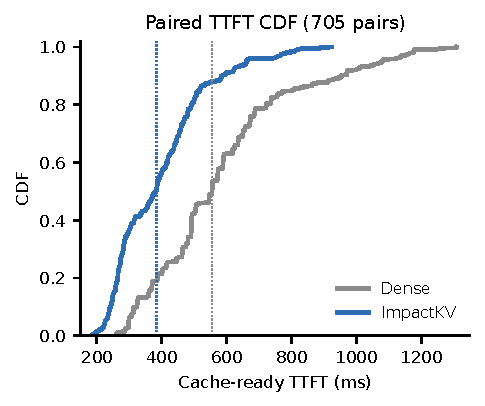
\includegraphics[width=\columnwidth]{figures/fig_ttft_cdf.pdf}
\caption{Empirical CDF of paired cache-ready TTFT (705 pairs, job 137185).
ImpactKV shifts the body and the tail: median $555{\to}383$\,ms, p90
$952{\to}586$\,ms, p99 $1178{\to}819$\,ms.}
\Description{Line chart CDF of Dense vs ImpactKV TTFT.}
\label{fig:ttft-cdf}
\end{figure}

\begin{figure}[t]
\centering
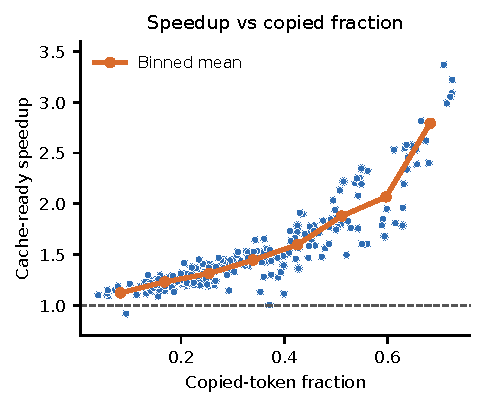
\includegraphics[width=\columnwidth]{figures/fig_copied_speedup.pdf}
\caption{Per-group cache-ready speedup versus copied-token fraction, with
a binned-mean line. Groups that copy more of the prompt are faster; the
headline $1.492\times$ is not a short-prompt artifact.}
\Description{Scatter of 235 groups plus binned-mean line.}
\label{fig:copied-speedup}
\end{figure}

The copy kernel did what the policy asked: 421 source pre-rotations, 1684
copies over four rounds per island (one warmup plus three measured), and
zero fallbacks. Mean cache-ready TTFT falls from $585.9$\,ms to
$392.7$\,ms ($1.492\times$ ratio of means). The paired median is
$555$\,ms versus $383$\,ms ($27.9\%$ saving); p90 is $952$\,ms versus
$586$\,ms; p99 is $1178$\,ms versus $819$\,ms. ImpactKV is faster on
$99.3\%$ of the 705 pairs. Per-group speedup has median $1.389\times$ and
ranges $0.918\times$--$3.369\times$. Groups with one, two, and three
admitted islands are $89$ / $106$ / $40$.

\subsection{Ablation of each module}

Job 139839 isolates M1 prefix reuse from M2 lossy copy on the 235-group
7B PLAN of Table~\ref{tab:eval-summary}, prefetch off. Speedups are versus
this campaign's Dense, not Table~\ref{tab:eval-summary}.
Figure~\ref{fig:prefix-on} and Table~\ref{tab:7b-prefix-on} report the
four arms. Prefix-only is $1.526\times$ (940 nonempty prefix hits, median
saving $32.9\%$, agreement $100\%$). Lossy-only is $1.408\times$ ($1684$
copies, median saving $23.7\%$, agreement $93.6\%$). Dual is
$2.120\times$ (median saving $55.4\%$, win rate $100\%$, agreement
$94.9\%$). The file-module increment given prefix is $1.390\times$
(dual / prefix-only) and is not mixed into Table~\ref{tab:eval-summary}.
Dual records 1126 copy events with 0 fallback. One-token agreement is
not Accuracy.

\begin{table}[t]
\centering
\small
\caption{Qwen2.5-Coder-7B-Instruct prefix-on increment on the 235-group
PLAN of job 137185 (job 139839). Speedups versus this campaign's Dense.
Prefetch off. Not Table~\ref{tab:eval-summary}, not the seven-group
dual-island table, not 30B.}
\label{tab:7b-prefix-on}
\resizebox{\columnwidth}{!}{%
\begin{tabular}{lrrrrrr}
\toprule
\textbf{Arm} & \textbf{TTFT} & \textbf{Med.\ save} & \textbf{Win} & \textbf{Agree} & \textbf{Prefix} & \textbf{Copy} \\
\midrule
Dense & $1.000\times$ & --- & --- & --- & --- & --- \\
prefix-only & $1.526\times$ & $32.9\%$ & $99.9\%$ & $100\%$ & $940$ & $0$ \\
lossy-only & $1.408\times$ & $23.7\%$ & $98.9\%$ & $93.6\%$ & $0$ & $1684$ \\
dual & $2.120\times$ & $55.4\%$ & $100\%$ & $94.9\%$ & $940$ & $1126$ \\
\bottomrule
\end{tabular}%
}
\end{table}

\begin{figure}[t]
\centering
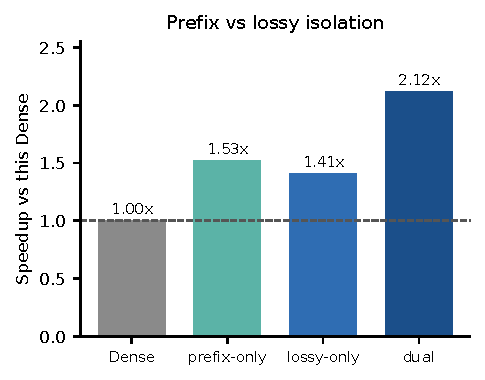
\includegraphics[width=\columnwidth]{figures/fig_prefix_on.pdf}
\caption{Prefix-on isolation on the 235-group PLAN (job 139839). Dual is
copy plus radix, not a prefetch win. Not
Table~\ref{tab:eval-summary}.}
\Description{Bar chart of Dense, prefix-only, lossy-only, and dual speedups.}
\label{fig:prefix-on}
\end{figure}

Job 137400 runs two policy clones on the same 7B prompts, Dense, and
SGLang executor as Table~\ref{tab:eval-summary}. KVCOMM-style admit
copies unconstrained $\Delta\neq 0$ exact spans (no file-module gate).
CacheBlend-style repair then Dense-recomputes $15\%$ of each such span
at the fusion boundary. Neither arm is the native CacheBlend or KVCOMM
serving stack. Table~\ref{tab:admit-ablation} is not
Table~\ref{tab:eval-summary}, not 30B, and not the seven-group
dual-island table.

Figure~\ref{fig:admit} and Table~\ref{tab:admit-ablation} are that
campaign. Unconstrained copy is faster because it moves more tokens:
KVCOMM-style $2.100\times$ cache-ready and CacheBlend-style $1.883\times$,
versus file-module $1.492\times$. Median paired saving is $27.9\%$ /
$50.9\%$ / $45.6\%$; win rates are $99.3\%$ / $99.9\%$ / $100\%$.
One-token agreement falls from $93.6\%$
($660/705$) to $89.4\%$ ($630/705$) and $91.9\%$ ($648/705$). On
$51$ pairs the file-module output matches Dense while KVCOMM-style
does not; the reverse is $21$ pairs. Those $51$ pairs are $17$ groups
with all three measured rounds. Table~\ref{tab:copier-extra-kinds}
decodes the extra tokens the file gate refused: tool observations,
tool commands, and assistant turns wrapped around the file island,
not a second admitted file module. On those $17$ groups every extra
token abuts a file island (campaign-wide $191{,}906/194{,}624$).
Figure~\ref{fig:motivation-extra} is the token-level reason: a campaign
total of $194{,}624$ extra unconstrained tokens, present in $235/235$
groups. That is why the headline stays coding-aware file-module copy
versus Dense, not a race on raw TTFT. We do not run a same-token 30B
CacheBlend or KVCOMM arm. A greedy longest-span copier on the 30B ids
(job 132385) is \emph{not a comparison target}: agreement falls from
$94.8\%$ to $87.1\%$.

\begin{table}[t]
\centering
\small
\caption{Decoded KVCOMM-only extra tokens (job 137400 PLANs). Leftover
prose is assistant; code dumps inside tool XML count as tool
observations. Not a new GPU arm, not admitted
\texttt{repository\_code}, and not Table~\ref{tab:eval-summary}.}
\label{tab:copier-extra-kinds}
\begin{tabular}{lrr}
\toprule
\textbf{Kind} & \textbf{Campaign} & \textbf{17 groups ($51$ pairs)} \\
\midrule
Tool observation & $117{,}965$ & $8{,}156$ \\
Tool command & $44{,}274$ & $2{,}517$ \\
Assistant turn & $28{,}471$ & $1{,}723$ \\
Chat marker & $3{,}914$ & $243$ \\
\midrule
Extra tokens & $194{,}624$ & $12{,}639$ \\
Abut a file island & $191{,}906$ & $12{,}639$ \\
\bottomrule
\end{tabular}
\end{table}

\begin{table}[t]
\centering
\small
\caption{Admit ablation: same-engine policy clones on
Qwen2.5-Coder-7B-Instruct SWE-bench prompts (job 137400). Not native
CacheBlend/KVCOMM stacks. Speedups versus this campaign's 7B Dense. Not
Table~\ref{tab:eval-summary}, not 30B, not the seven-group dual-island
table.}
\label{tab:admit-ablation}
\resizebox{\columnwidth}{!}{%
\begin{tabular}{lrrrrr}
\toprule
\textbf{Arm} & \textbf{TTFT} & \textbf{Med.\ save} & \textbf{Win} & \textbf{Agree} & \textbf{Copy} \\
\midrule
Dense & $1.000\times$ & --- & --- & --- & --- \\
File-module & $1.492\times$ & $27.9\%$ & $99.3\%$ & $93.6\%$ & $1684/1684$ \\
KVCOMM-style & $2.100\times$ & $50.9\%$ & $99.9\%$ & $89.4\%$ & $948/948$ \\
CacheBlend-style & $1.883\times$ & $45.6\%$ & $100\%$ & $91.9\%$ & $948/948$ \\
\bottomrule
\end{tabular}%
}
\end{table}

\begin{figure}[t]
\centering
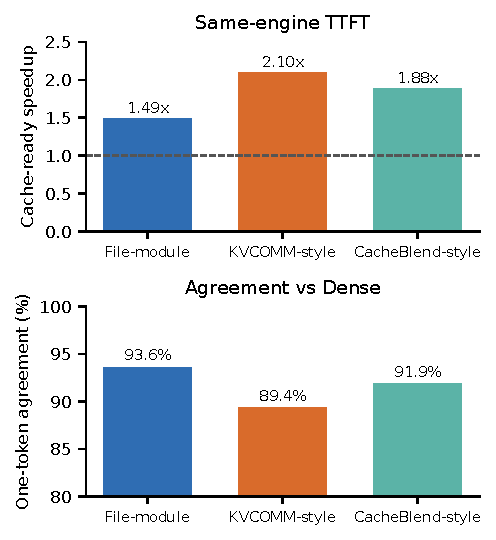
\includegraphics[width=\columnwidth]{figures/fig_admit.pdf}
\caption{Same-engine admit clones (job 137400). Unconstrained copy is
faster and agrees less. Not native CacheBlend/KVCOMM stacks and not
Table~\ref{tab:eval-summary}.}
\Description{Two-panel bar chart of cache-ready speedup and one-token agreement.}
\label{fig:admit}
\end{figure}

\subsection{Sensitivity}

Eligible islands are not tiny. Copied fraction grows with reconstructed
prompt length: $29\%$ below 3K tokens, $32\%$ in 3--5K, $34\%$ in 5--7K,
and $50\%$ at 7K and above (Table~\ref{tab:prompt-shape}). Position
deltas are strictly negative on this set (median $|\Delta| = 902$, range
$[82,7097]$): the same file appears earlier in the target than in the
source, which is exactly the rolling-history pattern prefix caches miss.

Figure~\ref{fig:eval-slices} splits the same 705 pairs four ways, derived
from job 137185, not a new GPU arm. Numeric companions are
Tables~\ref{tab:ablate-islands}, \ref{tab:ablate-delta},
and~\ref{tab:ablate-frac} in the appendix. Speedup grows with prompt
length: $1.28\times$ below 3K tokens, $1.43\times$ in 3--5K, $1.50\times$
in 5--7K, and $1.97\times$ at 7K and above. It also grows with admitted
files ($1.315\times$ / $1.492\times$ / $1.833\times$ for 1 / 2 / 3
islands) and with copied-token fraction (Q1 $1.196\times$, Q4
$2.116\times$). $|\Delta|$ is not the driver: a shift of $3000$ or more
is still $1.609\times$. Longer coding prompts and more copied file
bytes, not quiz-length prefill, are where the copy pays.

\begin{figure}[t]
\centering
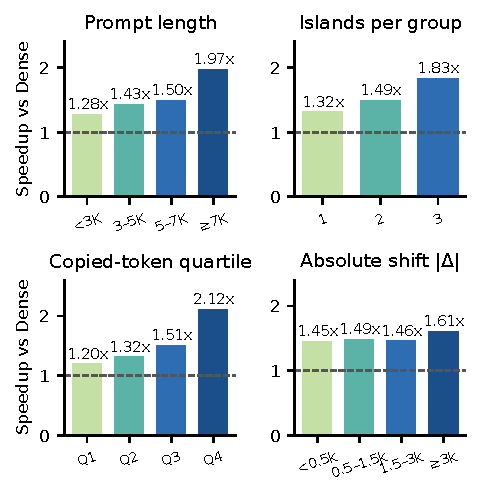
\includegraphics[width=\columnwidth]{figures/fig_slices.pdf}
\caption{Cache-ready TTFT speedup on the same 705 pairs (job 137185).
Not a new GPU arm and not Table~\ref{tab:eval-summary}.}
\Description{Four-panel bar chart: length, island count, copied-token quartile, and absolute shift.}
\label{fig:eval-slices}
\end{figure}

Of 115 unique source prompts, 101 appear in more than one target group
and 50 appear in five groups. That is why the page key includes prefix
and $\Delta$, not content hash alone. Forty-eight zero-shift islands were
dropped at plan time so this campaign cannot be credited to prefix cache.

\subsection{Output agreement is not Accuracy}

On the 705 measured pairs, $93.6\%$ of one-token outputs match Dense. The
artifact labels this field \texttt{not\_accuracy}. Official SWE-bench
resolved remains a live-agent, full-decode, hidden-test outcome. The
source expanded24 live-agent run recorded Dense $3/24$ and policy $5/24$
resolved (McNemar exact two-sided $p = 0.625$). That contrast is the
trajectory producer, not this replay, and it is not statistically
significant. This paper does not claim an official Accuracy win.
A content-only store on the same 7B PLAN mixed source-prefix pages
(job 137091) and agreement was $66.4\%$; Table~\ref{tab:eval-summary}
is the prefix-keyed campaign.

The 7B PLAN has 105 unique content hashes; 92 appear in more than one
group, and all 92 mix $\Delta$ inside the same 20-group restart window
(7 also mix source prefix). That is why the page key includes prefix
and $\Delta$. Replaying 30B token ids on 7B is invalid.
The seven-group dual-island isolation is Appendix~\ref{app:dual};
Table~\ref{tab:template-prefetch} stays job 119795.
